\chapter{Provázaní Backendu a Frontendu, API}

\section{Dokumentace online}
Aktuální dokumentace, tak aby mohla být časem aktualizována a mohli do ní
být připisovány další věci, se nachází na webu 
\href{http://quest.ms.mff.cuni.cz/prak/api/documentation}{quest.ms.mff.cuni.cz/prak/api/documentation}.
\\
Dokumentace je rozdělena na dvě části.
\\
\\
\textbf{Prvni cast} popisuje volani API. 
Kazda metoda (GET, POST atd.) ma svuj vlastni ucel
jez je popsan uvnitr, url, na kterou se dotazovat a mozne parametry.
Spolu s formatem requestu je i zde format odpovedi.
Podle kodu zjistime, jak uspesny byl nas pozadavek.
Kody jsou standartni podle "http status codes".
\begin{itemize}
	\item \textbf{2xx} Vsechno dopadlo dobre
	\item \textbf{4xx} Chyba je na strane klienta
	\item \textbf{5xx} Chyba je na strane serveru
\end{itemize}
V pripade uspechu (kod 200 - OK) se odesle odpoved na dotaz, nebo
nic pokud request nemel za funkci neco vracet. 
V pripade neuspechu pak v odpovedi najdeme zpravu o chybe ktera nastala.
Obvykle to u kodu 400 byva, ze odesilame duplicitni zaznam.
\\
\\
\textbf{Druha cast} popisuje strukturu schemat jednotlivych modelu\\
Jelikoz databaze ma datove formaty, zatimco JSON soubor ne (nebo alespon ne tak rozsahle)
musi i odesilana data mit spravny format, nebo alespon byt validni po automatickem
pretypovani.
Schema tvori JSON objekt popisujici schema.
pokud je datovy typ polozky objekt, bud se opravdu jedna o objekt, nebo
se jedna pouze o upresneni datoveho typu.
Klicovimy slovy jsou:
\begin{itemize}
	\item \textbf{type}: datovy typ
	\item \textbf{required}: true, pokud je tato polozka povinna
	\item \textbf{unique}: true, pokud se zadana hodnota, nesmi schodovat s jiz existujici polozkou v DB
	\item \textbf{ref}: nazev schematu, na ktery se ID odkazuje
	\item \textbf{refPath}: specialni ref, umoznujici uzivateli zadat i nazev schematu, vuci kteremu se odkazuje
\end{itemize}
Pokud je hodnota pouze string, pak je tato hodnota datovym typem.

\subsection{sowtware na online dokumentaci}
Pro moznost stazeni dokumentace a prohlizeni offline, je vse zabaleno do jednoho html souboru.
Uvnitr je zdrojovy kod programu, jez vykresluje stranku a zaroven data dokumentace samotne.
\\
Program vykresluje veskere polozky s daty dokumentace.
Bloky zdrojovych kodu jsou vysazeny monospacem a obarveny, aby uzivateli
poskytly rychlejsi orientaci v kodu.
\\\\
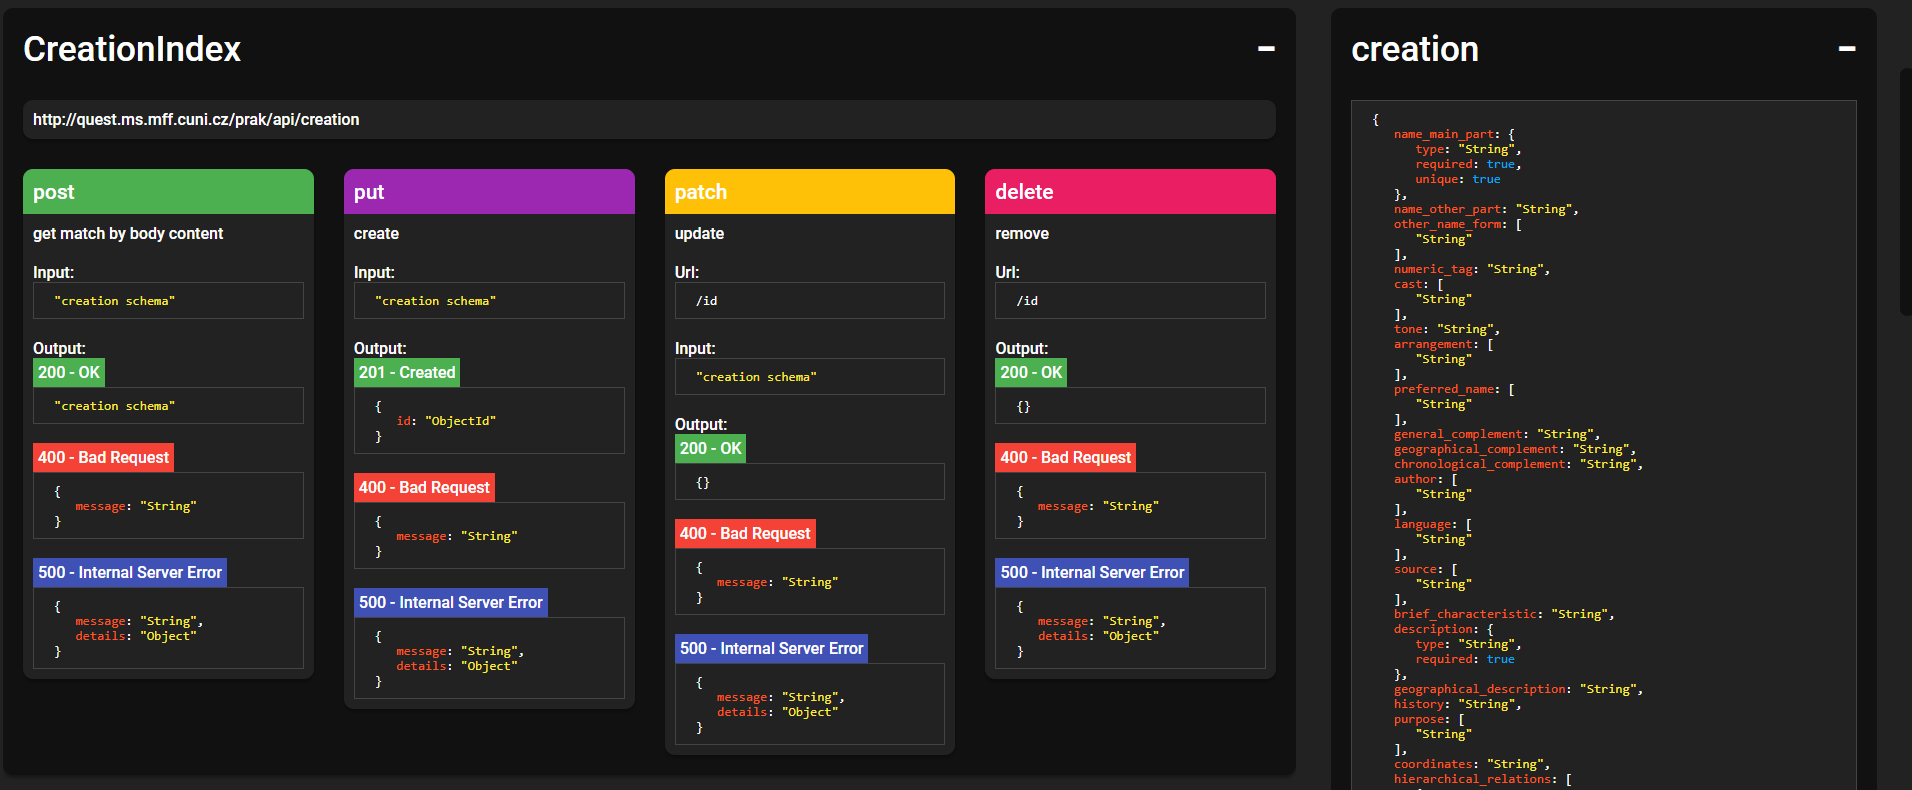
\includegraphics[width=\textwidth]{img/documentationPreview.PNG}


\section{Backend}
Na backendu je spusteny express server (bezici pod nodejs), ktery
zachytava requesty s url ...prak/api/... .
podle cesty, jez je uvedena za /api se request predava
prislosnemu routeru. Vyjimku tvori adresa .../api/documentation, ktera
rovnou preposila soubor s dokumentaci a neni tedy pro ziskani dokumentace
trba rozumet systemu hloubeji.
\\
\\
Pri prevzeti requestu jednim z mnoha routeru, se porovnava
typ requestu (POST, PUT atd.) a pripadne detaily cesty v url.
Pri plne nalezeni schody se provede overeni prav pokud je potreba.
Pokud request ma pozadovana opravneni je provedena prislusna funkce
a uzivateli je vracena odpoved / potvrzeni o uspechu.
V pripade ze request nema prislusna opravneni, je vracen kod 401.
V pripade ze se na serveru neco pokazi vrati se kod 400, nebo 500, podle typu problemu.

\section{API}
dostupne na adrese quest.ms.mff.cuni.cz/prak/api/

\subsection{Autentifikace}
S kazym requestem prichazi v hlavicce i cookies.
Pro autentifikaci pouzivam cookie se jmenem "sessionID".
Podle nej se najde prislusny uzivatel a porovnaji se jeho predava a
prava potrebna pro vykonani funkce. Pokud jsou prava nedostatecna, 
vrati se odpoved 401, v pripade spravneho opravneni, router vykona funkci
jez danemu requestu prislusi a pokud se nepokazi nic jineho, vrati validni odpoved.

\section{Frontend a volani API}
Jelikoz je cely projek zamyslen jako webova aplikace, nejstandartnejsi pouziti
je volani API pomoci JS funkce fetch(), coz je pouze zastita pro XMLHttpRequest.
Ale je mozne jej volat jakkoliv jinak, dokud to bude validni http request.

\subsection{Fetch}
Dokumentace metody: \href{https://developer.mozilla.org/en-US/docs/Web/API/Fetch_API}{mozilla}
\\
Priklad pouziti:
\\
\begin{lstlisting}[language=JavaScript]
	const url = "/prak/api/metadata" 
	fetch(url, {
		method: "POST",
		headers: { "Content-Type": "application/json" },
		body: JSON.stringify({ "name": "..." }),
	})
	.then(response => {
		if(!response.ok) throw response
		return response.json()
	})
	.then(response => {
		console.log(response)
	})
	.catch(error => {
		console.error(error)
	})
\end{lstlisting}

\subsection{Existujici programy pro praci a testovani APi}
Priklad volani pomoci programu Insomnia:
\\
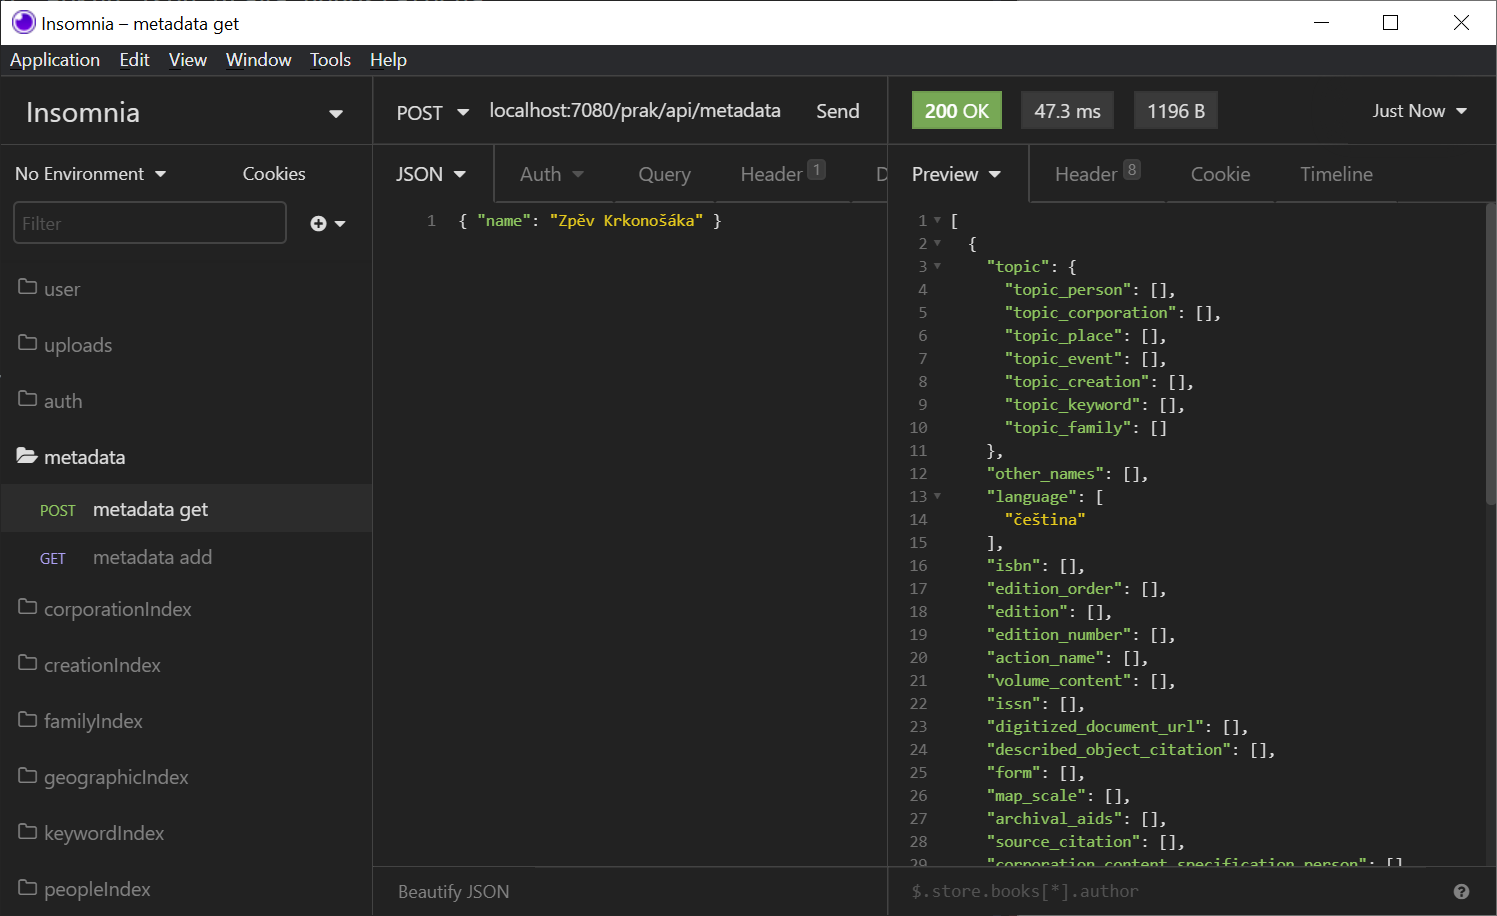
\includegraphics[width=\textwidth]{img/InsomniaExample.PNG}

